\documentclass{article}
%\documentclass[UTF8]{ctexart}
\usepackage{tikz}
\begin{document}
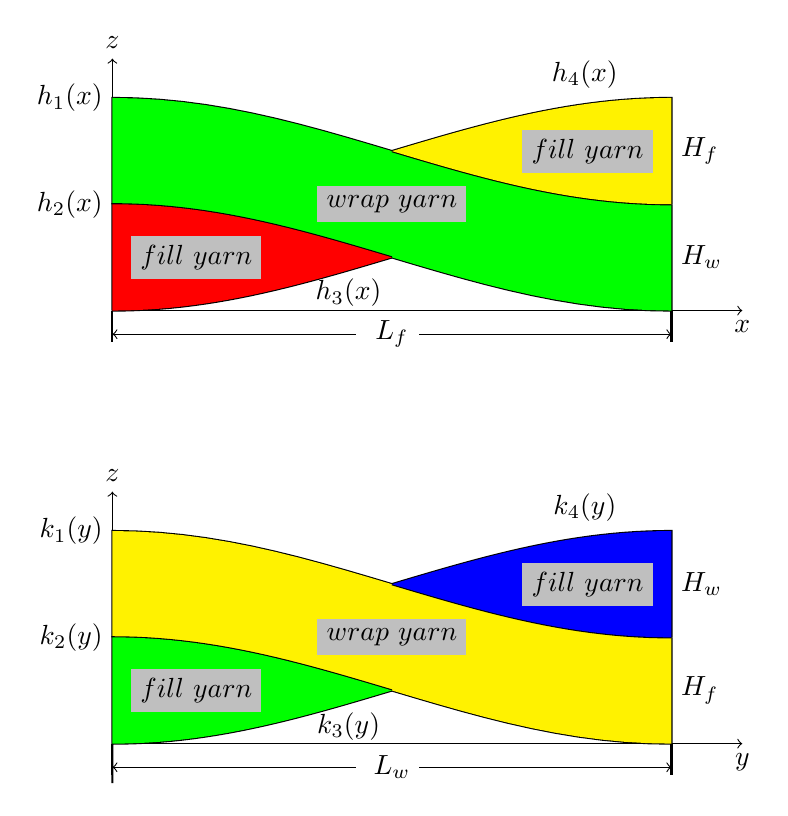
\begin{tikzpicture}

%x-z截面
%画出坐标轴
\draw[->] (0,0) -- (8,0) node[below]{$x$};
\draw[->] (0,0) -- (0,3.2) node[above]{$z$};
%画出经纱线和截面填充颜色
\draw[line width=0.8pt][black][domain=0:7.1] plot (\x, {1.35*0.5+1.35*0.5*cos(\x*pi/7.1 r)}) -- (7.1,1.35) [domain=7.1:0] plot (\x, {1.35*1.5+1.35*0.5*cos(\x*pi/7.1 r)}) -- (0,1.35); \fill[green][domain=0:7.1] plot (\x, {1.35*0.5+1.35*0.5*cos(\x*pi/7.1 r)}) -- (7.1,1.35) [domain=7.1:0] plot (\x, {1.35*1.5+1.35*0.5*cos(\x*pi/7.1 r)}) -- (0,1.35);
%画出纬纱线和截面填充颜色
\draw[line width=0.8pt][black][domain=0:3.55] plot (\x, {1.35*0.5-1.35*0.5*cos(\x*pi/7.1 r)}) -- (3.55,1.35*0.5) [domain=3.55:0] plot (\x, {1.35*0.5+1.35*0.5*cos(\x*pi/7.1 r)}) -- (0,0);
\fill[red][domain=0:3.55] plot (\x, {1.35*0.5-1.35*0.5*cos(\x*pi/7.1 r)}) -- (3.55,1.35*0.5) [domain=3.55:0] plot (\x, {1.35*0.5+1.35*0.5*cos(\x*pi/7.1 r)}) -- (0,0);
\draw[line width=0.8pt][black][domain=3.55:7.1] plot (\x, {1.35*1.5-1.35*0.5*cos(\x*pi/7.1 r)}) -- (7.1,1.35) [domain=7.1:3.55] plot (\x, {1.35*1.5+1.35*0.5*cos(\x*pi/7.1 r)}) -- (3.55,1.35*1.5);
\fill[yellow][domain=3.55:7.1] plot (\x, {1.35*1.5-1.35*0.5*cos(\x*pi/7.1 r)}) -- (7.1,1.35) [domain=7.1:3.55] plot (\x, {1.35*1.5+1.35*0.5*cos(\x*pi/7.1 r)}) -- (3.55,1.35*1.5);
%标注h1(x) h2(x) h3(x) h4(x) Hw Hf
\node[left] at (0,2.7) {$h_1(x)$};
\node[left] at (0,1.35) {$h_2(x)$};
\node[below] at (3,1.35*0.35+0.05){$h_3(x)$};
\node[above] at (6,1.35*2){$h_4(x)$};
\node[right] at (7.1,1.35*1.5){$H_f$};
\node[right] at (7.1,1.35*0.5){$H_w$};
%作Lf的标注
\draw [line width=0.8pt](0,0) -- (0,-0.4);
\draw [line width=0.8pt](7.1,0) -- (7.1,-0.4);
\draw[<-](0,-0.3)--(3.1,-0.3);
\draw[->](3.9,-0.3) -- (7.1,-0.3);
\node at (3.55,-0.3){$L_f$};
%\node[fill=lightgray] at (3.55,1.35){$wrap\,\,yarn$};
%\node[fill=lightgray] at (3.55*0.3,1.35*0.5){$fill\,\,yarn$};
%\node[fill=lightgray] at (3.55*1.7,1.35*1.5){$fill\,\,yarn$};
\node[fill=lightgray] at (3.55,1.35){$wrap\,\,yarn$};
\node[fill=lightgray] at (3.55*0.3,1.35*0.5){$fill\,\,yarn$};
\node[fill=lightgray] at (3.55*1.7,1.35*1.5){$fill\,\,yarn$};

%y-z截面
\draw[->] (0,-6+0.5) -- (8,-6+0.5) node[below]{$y$};
\draw[->] (0,-6+0.5) -- (0,3.2-6+0.5) node[above]{$z$};
%画出纬纱线和截面填充颜色
\draw[line width=0.8pt][black][domain=0:7.1] plot (\x, {1.35*0.5-6+0.5+1.35*0.5*cos(\x*pi/7.1 r)}) -- (7.1,1.35-6+0.5) [domain=7.1:0] plot (\x, {1.35*1.5-6+0.5+1.35*0.5*cos(\x*pi/7.1 r)}) -- (0,1.35-6+0.5);
\fill[yellow][domain=0:7.1] plot (\x, {1.35*0.5-6+0.5+1.35*0.5*cos(\x*pi/7.1 r)}) -- (7.1,1.35-6+0.5) [domain=7.1:0] plot (\x, {1.35*1.5-6+0.5+1.35*0.5*cos(\x*pi/7.1 r)}) -- (0,1.35-6+0.5);
%画出经纱线和截面填充颜色
\draw[line width=0.8pt][black][domain=0:3.55] plot (\x, {1.35*0.5-6+0.5-1.35*0.5*cos(\x*pi/7.1 r)}) -- (3.55,1.35*0.5-6+0.5) [domain=3.55:0] plot (\x, {1.35*0.5-6+0.5+1.35*0.5*cos(\x*pi/7.1 r)}) -- (0,-6);
\fill[green][domain=0:3.55] plot (\x, {1.35*0.5-6+0.5-1.35*0.5*cos(\x*pi/7.1 r)}) -- (3.55,1.35*0.5-6+0.5) [domain=3.55:0] plot (\x, {1.35*0.5-6+0.5+1.35*0.5*cos(\x*pi/7.1 r)}) -- (0,-6+0.5);
\draw[line width=0.8pt][black][domain=3.55:7.1] plot (\x, {1.35*1.5-6+0.5-1.35*0.5*cos(\x*pi/7.1 r)}) -- (7.1,1.35-6+0.5) [domain=7.1:3.55] plot (\x, {1.35*1.5-6+0.5+1.35*0.5*cos(\x*pi/7.1 r)}) -- (3.55,1.35*1.5-6+0.5);
\fill[blue][domain=3.55:7.1] plot (\x, {1.35*1.5-6+0.5-1.35*0.5*cos(\x*pi/7.1 r)}) -- (7.1,1.35-6+0.5) [domain=7.1:3.55] plot (\x, {1.35*1.5-6+0.5+1.35*0.5*cos(\x*pi/7.1 r)}) -- (3.55,1.35*1.5-6+0.5);
%标注h1(x) h2(x) h3(x) h4(x)
\node[left] at (0,2.7-6+0.5) {$k_1(y)$};
\node[left] at (0,1.35-6+0.5) {$k_2(y)$};
\node[below] at (3,1.35*0.35-6+0.05+0.5){$k_3(y)$};
\node[above] at (6,1.35*2-6+0.5){$k_4(y)$};
\node[right] at (7.1,1.35*1.5-5.5){$H_w$};
\node[right] at (7.1,1.35*0.5-5.5){$H_f$};
%作Lf的标注
\draw [line width=0.8pt](0,-6+0.5) -- (0,-0.4-6+0.5);
\draw [line width=0.8pt](7.1,-6+0.5) -- (7.1,-0.4-6+0.5);
\draw[<-](0,-0.3-6+0.5)--(3.1,-0.3-6+0.5);
\draw[->](3.9,-0.3-6+0.5) -- (7.1,-0.3-6+0.5);
\node at (3.55,-0.3-6+0.5){$L_w$};
\node[fill=lightgray] at (3.55,1.35-6+0.5){$wrap\,\,yarn$};
\node[fill=lightgray] at (3.55*0.3,1.35*0.5-6+0.5){$fill\,\,yarn$};
\node[fill=lightgray] at (3.55*1.7,1.35*1.5-6+0.5){$fill\,\,yarn$};
\end{tikzpicture}
\end{document}